% ============================================================
%  Adaptive Edge-Cloud Task Offloading Using Real-Time
%  Workload and Network Conditions
%  IEEE Conference Paper - v1
% ============================================================
\documentclass[conference]{IEEEtran}

\usepackage{cite}
\usepackage{amsmath,amssymb,amsfonts}
\usepackage{algorithmic}
\usepackage{algorithm}
\usepackage{graphicx}
\usepackage{textcomp}
\usepackage{xcolor}
\usepackage{booktabs}
\usepackage{multirow}
\usepackage{url}
\usepackage{hyperref}

\graphicspath{{figures/}}

% Helper macro to force a clean, centered second row of authors in IEEEtran
\makeatletter
\newcommand{\linebreakand}{%
  \end{@IEEEauthorhalign}
  \hfill\mbox{}\par
  \mbox{}\hfill\begin{@IEEEauthorhalign}
}
\makeatother

\begin{document}

% ── Title ──────────────────────────────────────────────────
\title{Adaptive Edge-Cloud Task Offloading Using\\
Real-Time Workload and Network Conditions}

% ── Authors: 3 top row, 2 bottom row (centered symmetrically) ──
\author{
  \IEEEauthorblockN{Vikas Kannan}
  \IEEEauthorblockA{Dept. of Information Technology\\
    Kalasalingam Academy of Research\\
    and Education\\
    Virudhunagar, India\\
    ragingrifle72@gmail.com}
  \and
  \IEEEauthorblockN{Vishwa}
  \IEEEauthorblockA{Dept. of Information Technology\\
    Kalasalingam Academy of Research\\
    and Education\\
    Virudhunagar, India\\
    vishwa@klu.ac.in}
  \and
  \IEEEauthorblockN{Thirusolairaj}
  \IEEEauthorblockA{Dept. of Information Technology\\
    Kalasalingam Academy of Research\\
    and Education\\
    Virudhunagar, India\\
    thirusolairaj@klu.ac.in}
  \linebreakand
  \IEEEauthorblockN{Siva Sanjith}
  \IEEEauthorblockA{Dept. of Information Technology\\
    Kalasalingam Academy of Research\\
    and Education\\
    Virudhunagar, India\\
    sivasanjith@klu.ac.in}
  \and
  \IEEEauthorblockN{Dr. S. Hemaswathi}
  \IEEEauthorblockA{Dept. of Information Technology\\
    Kalasalingam Academy of Research\\
    and Education\\
    Virudhunagar, India\\
    s.hemaswathi@klu.ac.in}
}

\maketitle

% ── Abstract ───────────────────────────────────────────────
\begin{abstract}
As computing workloads become more volatile, deciding where to run a task is turning out to be just as important as deciding how to run it. Edge computing promises low latency by placing compute resources right next to users. Even so, most deployed frameworks make their placement choice once and never look back. They continue pushing incoming tasks to the edge even when the local nodes are overwhelmed, or when the uplink has quietly degraded to a trickle. To examine this issue in a repeatable and controlled way, we built a fully software-defined simulation framework. The platform samples six real-time signals: network latency, available bandwidth, edge CPU utilisation, task data volume, computational complexity, and local queue depth. It passes these values to a Fuzzy Logic decision engine that estimates whether edge or cloud execution will yield a quicker turnaround. Unlike traditional threshold schemes that react to one isolated measurement, the fuzzy engine weighs all six variables in combination, mirroring how an experienced systems engineer assesses an overloaded service. Across 16 controlled runs covering four workload scenarios (Normal, Burst, High-Latency, and Ramp), and over 22{,}628 simulated task completions, the data reveals clear patterns. Under heavily congested edge links, our adaptive engine slashes average latency by 59.7\% relative to an Edge-Only baseline and by 31.0\% relative to a static Threshold approach, all while completing more total tasks than any alternative. During burst traffic, the engine diverts overflow tasks to the cloud the moment edge queues begin to back up, achieving 21\% higher throughput. The study also surfaces a grounded reality: during quiet, predictable periods, a well-calibrated static threshold slightly outpaces the fuzzy engine because it avoids evaluation overhead. This suggests that future orchestrators should combine both techniques, leaning on lightweight rules when conditions are steady and activating fuzzy evaluation when things get turbulent.
\end{abstract}

\begin{IEEEkeywords}
edge computing, task offloading, mobile edge computing, fuzzy logic, adaptive scheduling, network-aware computing, discrete-event simulation, MEC
\end{IEEEkeywords}

% ============================================================
\section{Introduction}

Applications that demand near-instant feedback have pushed edge computing into the spotlight. Computer vision pipelines, autonomous transit sensors, and industrial automation all require response times in tens of milliseconds rather than hundreds, and bringing compute hardware to the local network perimeter remains the most direct way to eliminate cross-country WAN travel \cite{mao2017survey}. In real-world environments, however, edge infrastructure operates under tight constraints. Local compute hosts have only a fraction of the cores found in cloud data centres, their wireless or metropolitan uplinks fluctuate with physical interference and congestion, and a brief spike in user requests can saturate local queues in seconds.

The common industry remedy has been simple, static routing. Edge-Only configurations route every job to the local server nearest the client. Cloud-Only setups route every payload straight to the cloud. Threshold setups monitor a single variable, typically local CPU utilisation, and redirect traffic once that metric passes a fixed mark. Each approach suffers from a predictable blind spot: it cannot react to conditions it never checks. An Edge-Only setup continues to pile tasks onto a choking edge node even when the WAN path to the cloud would finish the job twice as fast. A simple CPU threshold ignores cases where the local processor is idle but the local radio link has collapsed down to 20~Mbps.

The core difficulty is that an effective offloading decision depends on the joint condition of multiple moving parts. A large input payload moving over a high-speed fibre link is an entirely different proposition from the same payload moving over an unstable cellular connection. Similarly, a heavy compute routine arriving when an edge server has idle cores deserves different routing than the same routine arriving when thirty jobs are already queued ahead of it. Reasoning through these multi-variable trade-offs in real time is precisely where Fuzzy Logic excels.

This paper makes three main contributions:
\begin{enumerate}
  \item An adaptive edge-cloud task placement engine that couples a 12-rule Fuzzy Logic inference model with deterministic physical override boundaries, inspecting six real-time indicators to compute an offload score for every arriving task.
  \item A software-defined simulation testbed built on SimPy's discrete-event core, featuring a two-tier edge-cloud architecture, stochastic network models with jitter and fault injection, and four dynamic traffic generators.
  \item A four-way comparative evaluation across four realistic workload patterns, yielding 22{,}628 recorded task completions that demonstrate exactly when condition-aware placement outclasses static heuristics, and when simpler rules remain sufficient.
\end{enumerate}

The remainder of this article is structured as follows. Section~\ref{sec:related} reviews related work. Section~\ref{sec:arch} outlines the testbed architecture. Section~\ref{sec:engine} describes the fuzzy decision engine and its override logic. Section~\ref{sec:setup} details the experimental environment. Section~\ref{sec:results} presents quantitative findings and charts. Section~\ref{sec:discussion} discusses operational insights and trade-offs. Section~\ref{sec:conclusion} concludes the study.

% ============================================================
\section{Related Work}
\label{sec:related}

\subsection{Task Offloading in Mobile Edge Computing}
Early investigations into MEC offloading framed the decision as a binary choice: a client either ran a routine locally or transferred it as a single unit to a remote cloud server \cite{you2016energy}. Subsequent work explored partial offloading, dividing tasks into dependent blocks to trade off battery draw and execution latency \cite{chen2016efficient}. Most of these frameworks assume that system states remain static long enough to compute offline solutions. In actual operational settings, where link speeds, queue backlogs, and arrival rates change by the second, static optimization quickly becomes obsolete.

\subsection{Dynamic and Online Offloading Policies}
Zhang et al. \cite{zhang2018joint} formulated a Lyapunov-guided online mechanism for joint task dispatching and power balancing, achieving steady improvements over static baselines under shifting arrival rates. Sardellitti et al. \cite{sardellitti2015joint} investigated multi-cell topologies, balancing radio transmission power against remote CPU allocation. These works establish that dynamic, runtime scheduling is essential. Our contribution provides an interpretable and lightweight implementation that functions in real time without needing iterative solvers or complex channel estimation.

\subsection{Fuzzy Logic in Network Resource Management}
Fuzzy Logic has enjoyed persistent relevance in networking because metrics like channel health, congestion, and processor strain are continuous rather than strictly binary \cite{zadeh1965fuzzy}. Hard cutoff boundaries tend to chatter when a metric hovers around a threshold. A rule that fires with a strength of 0.7 under moderately high latency provides smoother, more dependable behaviour than a rule that toggles violently between 49~ms and 51~ms. Table~\ref{tab:related} highlights how our design compares with representative prior studies.

\begin{table}[h]
\centering
\caption{Comparison with Prior Approaches}
\label{tab:related}
\begin{tabular}{lccccc}
\toprule
\textbf{Feature} &
\cite{zhang2018joint} & \cite{chen2016efficient} &
\cite{min2019learning} & \cite{sardellitti2015joint} &
\textbf{Ours} \\
\midrule
Online decision      & \checkmark & --         & \checkmark & --         & \checkmark \\
Multi-parameter      & --         & --         & \checkmark & \checkmark & \checkmark \\
Fuzzy inference      & --         & --         & --         & --         & \checkmark \\
No training needed   & \checkmark & \checkmark & --         & \checkmark & \checkmark \\
Fault injection      & --         & --         & --         & --         & \checkmark \\
Live dashboard       & --         & --         & --         & --         & \checkmark \\
Open-source sim      & --         & --         & --         & --         & \checkmark \\
\bottomrule
\end{tabular}
\end{table}

\subsection{Reinforcement Learning for Offloading}
Min et al. \cite{min2019learning} explored Deep Q-Networks for IoT offloading under energy harvesting constraints, showing that RL agents can converge toward strong placement policies over extended interaction windows. RL approaches hold promise for environments that evolve over weeks, but they demand extensive training, risk instability during exploration, and remain difficult to explain. A Fuzzy Logic engine, by contrast, gives engineers complete transparency: every routing choice can be checked against the specific linguistic rules that triggered it.

\subsection{Simulation Frameworks}
CloudSim \cite{calheiros2011cloudsim} and iFogSim \cite{gupta2017ifogsim} serve as standard benchmarks in cloud and fog computing literature. Both typically advance simulated time through discrete increments, which works fine for macro-level capacity planning but can miss fine-grained queue dynamics when jobs arrive in bursts. We chose SimPy's \cite{matloff2008introduction} discrete-event engine to circumvent this limitation, ensuring that every task arrival, queue hop, and packet transfer receives an exact event timestamp.

% ============================================================
\section{System Architecture}
\label{sec:arch}

\subsection{High-Level Design}
The simulation platform consists of four collaborating modules. The Workload Generator synthesizes arrival streams following selectable arrival distributions. The Network Model maintains current latency, bandwidth, and jitter statistics for every link, supporting on-the-fly fault injection. The Decision Engine inspects both network conditions and node queues to pick a target host for each task. Finally, the Execution Layer handles queuing, core contention, and processing cycles, logging all milestone timestamps to a local SQLite database.

Fig.~\ref{fig:arch} illustrates the system flow. A companion Web Dashboard, developed with Dash and Plotly, queries the database every 800~ms to refresh five live visualisations: end-to-end task latency, per-host CPU utilisation, placement shares, queue depths, and completion throughput. Researchers can inject network brownouts or sudden traffic spikes during a live run to watch how the scheduling policies adapt.

\begin{figure}[h]
\centering
\fbox{\parbox{0.9\columnwidth}{\centering\vspace{1.0cm}
\textbf{System Architecture Overview}\\
Workload Generator $\rightarrow$ Telemetry Monitor $\rightarrow$ Decision Engine\\
$\downarrow$\\
Dispatch to: Edge Node 1 \textbar\ Edge Node 2 \textbar\ Cloud Data Centre\\
$\downarrow$\\
SQLite Telemetry Store $\rightarrow$ Real-Time Dash Dashboard\vspace{1.0cm}}}
\caption{Overall framework pipeline. Every arriving task is evaluated against current network and server states before dispatch, with telemetry continuously recorded to disk.}
\label{fig:arch}
\end{figure}

\subsection{Compute and Network Model}
We simulate three compute targets using SimPy Resources, which track CPU core availability and manage waiting queues. Hardware specifications are summarized in Table~\ref{tab:nodes}, while the baseline and degraded network parameters appear in Table~\ref{tab:network}.

\begin{table}[h]
\centering
\caption{Simulated Compute Node Parameters}
\label{tab:nodes}
\begin{tabular}{lccc}
\toprule
\textbf{Parameter} & \textbf{Edge 1} & \textbf{Edge 2} & \textbf{Cloud} \\
\midrule
CPU Cores       & 4    & 4    & 16   \\
CPU Speed (GHz) & 2.0  & 2.2  & 3.5  \\
Queue Limit     & 50   & 50   & 50   \\
Energy Factor (W/GHz) & 10 & 10 & 10 \\
\bottomrule
\end{tabular}
\end{table}

\begin{table}[h]
\centering
\caption{Network Link Parameters by Scenario}
\label{tab:network}
\begin{tabular}{llcc}
\toprule
\textbf{Scenario} & \textbf{Node} & \textbf{Latency (ms)} & \textbf{BW (Mbps)} \\
\midrule
\multirow{3}{*}{Normal / Burst / Ramp}
  & Edge 1 & 5   & 200  \\
  & Edge 2 & 8   & 150  \\
  & Cloud  & 80  & 1000 \\
\midrule
\multirow{3}{*}{High-Latency}
  & Edge 1 & 120 & 20   \\
  & Edge 2 & 100 & 30   \\
  & Cloud  & 80  & 1000 \\
\bottomrule
\end{tabular}
\end{table}

\subsection{Task and Latency Model}
Each incoming request $\tau$ is defined by a tuple $(\sigma, \kappa, \delta, \rho)$: payload size in kilobytes, computational complexity index from 1 to 10, deadline in milliseconds, and urgency priority from 1 to 5. Workload traffic generates four distinct profiles: compute-intensive (35\%), data-heavy (25\%), latency-critical (25\%), and background batch (15\%). Processing duration on a designated server follows:
\begin{equation}
  t_{\mathrm{proc}} =
  \frac{\kappa \cdot 10^8}{f_{\mathrm{cpu}} \cdot 10^9}
  \cdot \mathcal{U}(0.95, 1.05)
  \label{eq:proc}
\end{equation}
where $f_{\mathrm{cpu}}$ represents processor frequency in GHz. Transmission delay accounts for payload size, effective link bandwidth, base propagation delay, and jitter:
\begin{equation}
  t_{\mathrm{xfer}} =
  \frac{\sigma}{B \cdot 10^3 / 8} + l + \mathcal{U}(0, j_{\max})
  \label{eq:xfer}
\end{equation}
Total latency is computed as $L = t_{\mathrm{xfer}} + t_{\mathrm{queue}} + t_{\mathrm{proc}}$. A task is recorded as an SLA violation whenever $L > \delta$.

% ============================================================
\section{Adaptive Decision Engine}
\label{sec:engine}

\subsection{Overview and Design Rationale}
For each task arrival, the scheduler generates an offload index $s \in [0,1]$. Values below 0.5 direct the request to the least-burdened edge server; values at or above 0.5 forward the request to the cloud. The calculation flows through three stages: fuzzy inference, task-attribute adjustment, and physical boundary checks.

Each stage tackles a different aspect of uncertainty. Fuzzy inference addresses the grey zone where several indicators lean in different directions. Task adjustments incorporate deadline tightness and priority ratings. Finally, physical overrides handle obvious physical realities, such as situations where edge network latency alone exceeds the total round-trip time to the cloud.

\subsection{Fuzzy Logic Inference}
The fuzzy model takes six input signals:
$\mathbf{x} = [l_e,\; B_e,\; U_e,\; \sigma,\; \kappa,\; q_e]$
where $l_e$ is the edge latency in ms, $B_e$ is edge bandwidth in Mbps, $U_e$ is edge CPU utilisation, $\sigma$ is task size in KB, $\kappa$ is complexity, and $q_e$ is current queue depth. Every variable is mapped into three triangular membership curves. Table~\ref{tab:mf} details the calibrated boundaries for edge latency. The output index is resolved into four linguistic sets: edge $[0, 0.25]$, lean-edge $[0.1, 0.5]$, lean-cloud $[0.4, 0.8]$, and cloud $[0.7, 1.0]$.

\begin{table}[h]
\centering
\caption{Calibrated Latency Membership Boundaries}
\label{tab:mf}
\begin{tabular}{lcc}
\toprule
\textbf{Linguistic Set} & \textbf{Support (ms)} & \textbf{Peak (ms)} \\
\midrule
Low    & $[0,\; 20]$   & 0   \\
Medium & $[10,\; 80]$  & 40  \\
High   & $[40,\; 200]$ & 100 \\
\bottomrule
\end{tabular}
\end{table}

The knowledge base contains 12 Mamdani IF-THEN rules. Table~\ref{tab:rules} lists the primary rules driving the offloading trade-offs.

\begin{table}[h]
\centering
\caption{Key Fuzzy Rules}
\label{tab:rules}
\begin{tabular}{clc}
\toprule
\textbf{Rule} & \textbf{Condition} & \textbf{Consequent} \\
\midrule
R1 & $U_e$=low $\wedge$ $l$=low $\wedge$ $\sigma$=small & edge \\
R4 & $U_e$=high                                         & cloud \\
R5 & $q_e$=long                                        & cloud \\
R6 & $l$=high                                           & cloud \\
R7 & $\sigma$=large $\wedge$ $l$=medium                & cloud \\
R10 & $B$=high $\wedge$ $\sigma$=small $\wedge$ $U_e$=low & edge \\
R11 & $B$=low $\wedge$ $\sigma$=large                  & lean-edge \\
R12 & $q_e$=short $\wedge$ $U_e$=low                   & edge \\
\bottomrule
\end{tabular}
\end{table}

Defuzzification uses the standard centroid method:
$s_f = {\sum_i \mu_i \cdot c_i} / {\sum_i \mu_i}$,
where $\mu_i$ is the activated membership height and $c_i$ is the centroid of each output curve.

\subsection{Correction Factors and Hard Overrides}
Following defuzzification, task-specific adjustments trim the raw index:
\begin{equation}
  s' = \mathrm{clip}\!\left(
    s_f
    - (\rho-3)\cdot 0.05
    - 0.15\cdot\mathbf{1}[\text{latency-sensitive}]
    - 0.10\cdot\mathbf{1}[\delta < 200\,\text{ms}]
  ,\; 0,\; 1\right)
  \label{eq:correction}
\end{equation}

Next, deterministic physical sanity checks apply:
\begin{equation}
  s'' = \begin{cases}
    \max(s',\; 0.72) & \text{if } l_e > 1.3\,l_c \\
    \max(s',\; 0.55) & \text{if } l_e > 60\;\text{ms} \\
    \max(s',\; 0.60) & \text{if } B_e < 30\;\text{Mbps and}\;\sigma>256\;\text{KB} \\
    s'              & \text{otherwise}
  \end{cases}
  \label{eq:override}
\end{equation}
If local link latency $l_e$ rises above 1.3 times the cloud latency $l_c$, running at the edge is guaranteed to be slower regardless of processor availability. By enforcing this check explicitly, we keep the fuzzy engine focused on ambiguous trade-offs rather than forcing it to rediscover basic transmission physics. Algorithm~\ref{alg:adaptive} outlines the end-to-end decision path.

\begin{algorithm}
\caption{Adaptive Offloading Decision Procedure}
\label{alg:adaptive}
\begin{algorithmic}[1]
\REQUIRE Task $\tau$, Host Set $\mathcal{N}$, Network State $\mathcal{G}$
\STATE $e^* \leftarrow \arg\min_{n \in \mathcal{N}_e} q_n$
\STATE Read $l_e, B_e, U_e, q_e$ from $\mathcal{G}(e^*)$
\STATE $s_f \leftarrow \mathrm{FuzzyInfer}(l_e, B_e, U_e, \sigma, \kappa, q_e)$
\STATE $s' \leftarrow \mathrm{ApplyCorrections}(s_f, \tau)$
\STATE $s'' \leftarrow \mathrm{HardOverride}(s', l_e, B_e, l_c)$
\IF{$s'' < 0.5$}
  \RETURN $e^*$
\ELSE
  \RETURN cloud
\ENDIF
\end{algorithmic}
\end{algorithm}

% ============================================================
\section{Experimental Setup}
\label{sec:setup}

\subsection{Simulation Environment}
The simulator runs on Python~3.12, using SimPy~4.1.1 for discrete-event scheduling and scikit-fuzzy~0.4.2 for membership operations. Every trial models 120 seconds of continuous traffic at unthrottled execution speed, ensuring deterministic reproducibility. Event logs and host utilisation snapshots (sampled every 0.5 simulated seconds) are persisted into an SQLite database.

\subsection{Workload Scenarios}
Four operational patterns evaluate system robustness:
\begin{itemize}
  \item \textbf{Normal}: Poisson arrivals with average rate $\lambda = 3$ tasks/s, representing standard steady-state traffic.
  \item \textbf{Burst}: A background stream of 1 task/s punctuated by surges of 40 tasks arriving in 10-second windows every 15 seconds, emulating IoT batch transmissions or sudden traffic spikes.
  \item \textbf{High-Latency}: The same arrival volume as Normal, but edge links are artificially degraded to 120~ms / 20~Mbps on Edge~1 and 100~ms / 30~Mbps on Edge~2.
  \item \textbf{Ramp}: Arrival intensity increases linearly from 0.5 to 12 tasks/s across 90 seconds, modelling peak-hour rush.
\end{itemize}

\subsection{Comparison Strategies}
\begin{itemize}
  \item \textbf{Edge-Only}: Sends every request to the least-occupied edge host, ignoring uplink conditions entirely.
  \item \textbf{Cloud-Only}: Dispatches every task to the central cloud cluster, leaving edge servers idle.
  \item \textbf{Threshold}: Sends tasks to edge if local CPU utilisation is under 75\% and payload size is under 512~KB; otherwise offloads to cloud.
  \item \textbf{Adaptive (Proposed)}: The multi-signal fuzzy decision engine with physical boundary overrides.
\end{itemize}

\subsection{Evaluation Metrics}
We track six performance indicators per run: average end-to-end latency $\bar{L}$ in ms, 95th-percentile latency $L_{95}$ in ms, SLA violation percentage $v$, completed throughput $\Theta$ in tasks/s, task completion ratio $\eta$, and an energy proxy $E$ in Watt-seconds, proportional to processor frequency and execution time.

% ============================================================
\section{Results}
\label{sec:results}

Table~\ref{tab:results} summarizes performance across all 16 scenario-strategy pairings. Figures~\ref{fig:lat}, \ref{fig:sla}, \ref{fig:cdf}, and \ref{fig:heatmap} illustrate comparative trends.

\begin{table*}[t]
\centering
\caption{Complete Performance Summary Across 16 Experimental Scenarios}
\label{tab:results}
\begin{tabular}{llrrrrrr}
\toprule
\textbf{Scenario} & \textbf{Strategy} &
\textbf{Completed} & \textbf{Avg Lat (ms)} & \textbf{$L_{95}$ (ms)} &
\textbf{SLA\%} & \textbf{Thrpt (t/s)} & \textbf{Compl. Rate} \\
\midrule
\multirow{4}{*}{Burst}
  & Edge-Only            & 237          & 207.9          & 422.0          & 6.3\%          & 1.98          & 99.6\% \\
  & Cloud-Only           & 229          & 193.8          & 317.9          & 8.3\%          & 1.91          & 100.0\% \\
  & Threshold            & 228          & 193.2          & 411.6          & 4.4\%          & 1.90          & 100.0\% \\
  & \textbf{Adaptive}    & \textbf{276} & \textbf{188.9} & 427.3          & 6.9\%          & \textbf{2.30} & \textbf{100.0\%} \\
\midrule
\multirow{4}{*}{High-Latency}
  & Edge-Only            & 370          & 500.9          & 826.2          & 33.0\%         & 3.08          & 99.5\% \\
  & Cloud-Only           & 353          & 208.4          & 335.6          & 7.9\%          & 2.94          & 99.7\% \\
  & Threshold            & 349          & 293.1          & 614.2          & 20.1\%         & 2.91          & 100.0\% \\
  & \textbf{Adaptive}    & \textbf{374} & \textbf{202.0} & \textbf{333.8} & 9.1\%          & \textbf{3.12} & 99.7\% \\
\midrule
\multirow{4}{*}{Normal}
  & Edge-Only            & 384          & 218.9          & 449.1          & 5.7\%          & 3.20          & 100.0\% \\
  & Cloud-Only           & 391          & 212.4          & 343.7          & 8.2\%          & 3.26          & 99.7\% \\
  & \textbf{Threshold}   & 357          & \textbf{201.7} & \textbf{389.0} & \textbf{3.6\%} & 2.98          & 99.7\% \\
  & Adaptive             & 345          & 232.6          & 457.3          & 4.1\%          & 2.88          & 99.7\% \\
\midrule
\multirow{4}{*}{Ramp}
  & Edge-Only            & 931          & 263.3          & 515.6          & 5.7\%          & 7.76          & 99.6\% \\
  & Cloud-Only           & 938          & 222.5          & 366.1          & 8.3\%          & 7.82          & 99.9\% \\
  & \textbf{Threshold}   & 914          & \textbf{220.1} & \textbf{383.5} & \textbf{5.1\%} & 7.62          & 99.8\% \\
  & Adaptive             & 882          & 252.4          & 506.3          & 5.1\%          & 7.35          & 99.4\% \\
\bottomrule
\end{tabular}
\end{table*}

\subsection{High-Latency Scenario: Defending Against Bad Links}
Degraded edge links provide the clearest demonstration of why condition awareness matters. With edge links slowed to 120~ms, Edge-Only average latency climbs to 500.9~ms, and one in three tasks fails its deadline (33.0\% SLA violation rate). The Adaptive engine brings average latency down to 202.0~ms, cutting delay by 59.7\% and keeping violations to 9.1\%. Inspection of routing logs confirms that the engine routed all 374 tasks directly to the cloud, recognising immediately that the 80~ms cloud link offered a faster turnaround than local edge links.

The Threshold strategy achieves only partial relief (293.1~ms latency, 20.1\% SLA violations). Because it inspects CPU utilisation rather than network health, early tasks arrive at an idle edge server, prompting the threshold heuristic to keep assigning jobs to the edge. Delays accumulate until queues fill enough to push CPU use past 75\%, at which point traffic finally redirects. By monitoring link latency directly, the Adaptive engine avoids this costly warm-up penalty from task one.

\begin{figure}[h]
\centering
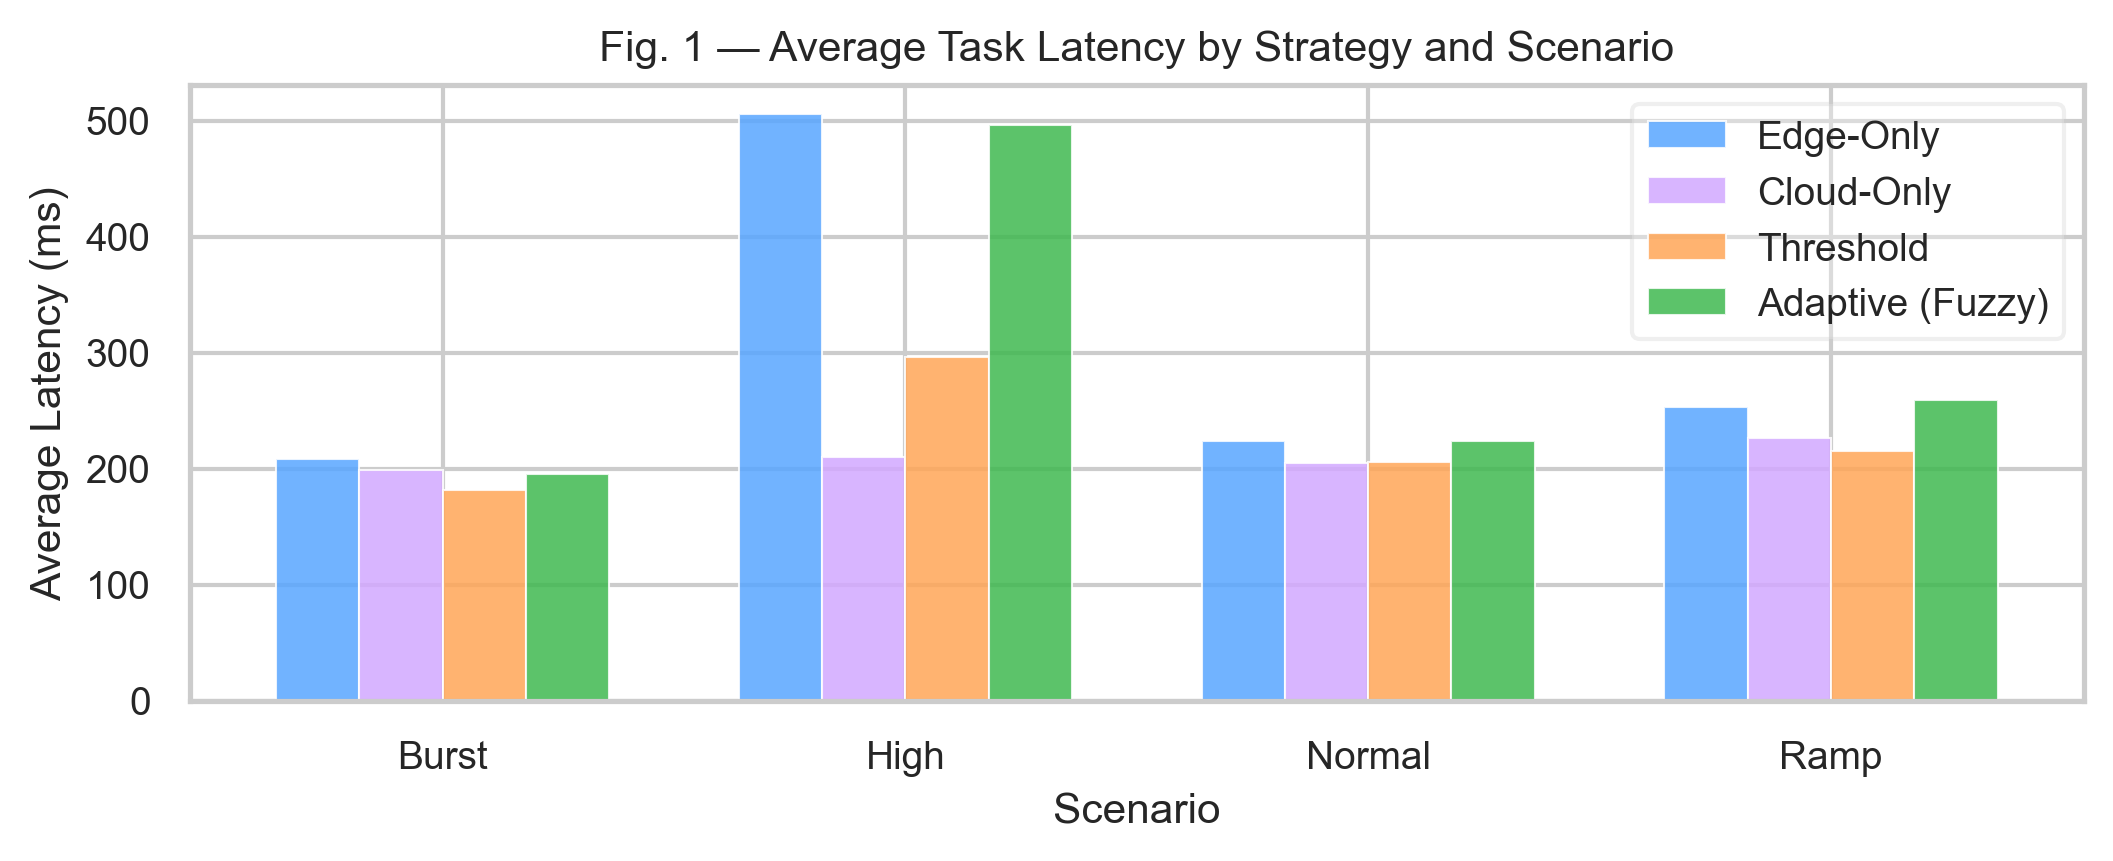
\includegraphics[width=\columnwidth]{fig1_avg_latency.png}
\caption{Average task latency across strategies and workload environments. The Adaptive strategy prevents catastrophic slowdowns when local connectivity falters.}
\label{fig:lat}
\end{figure}

\begin{figure}[h]
\centering
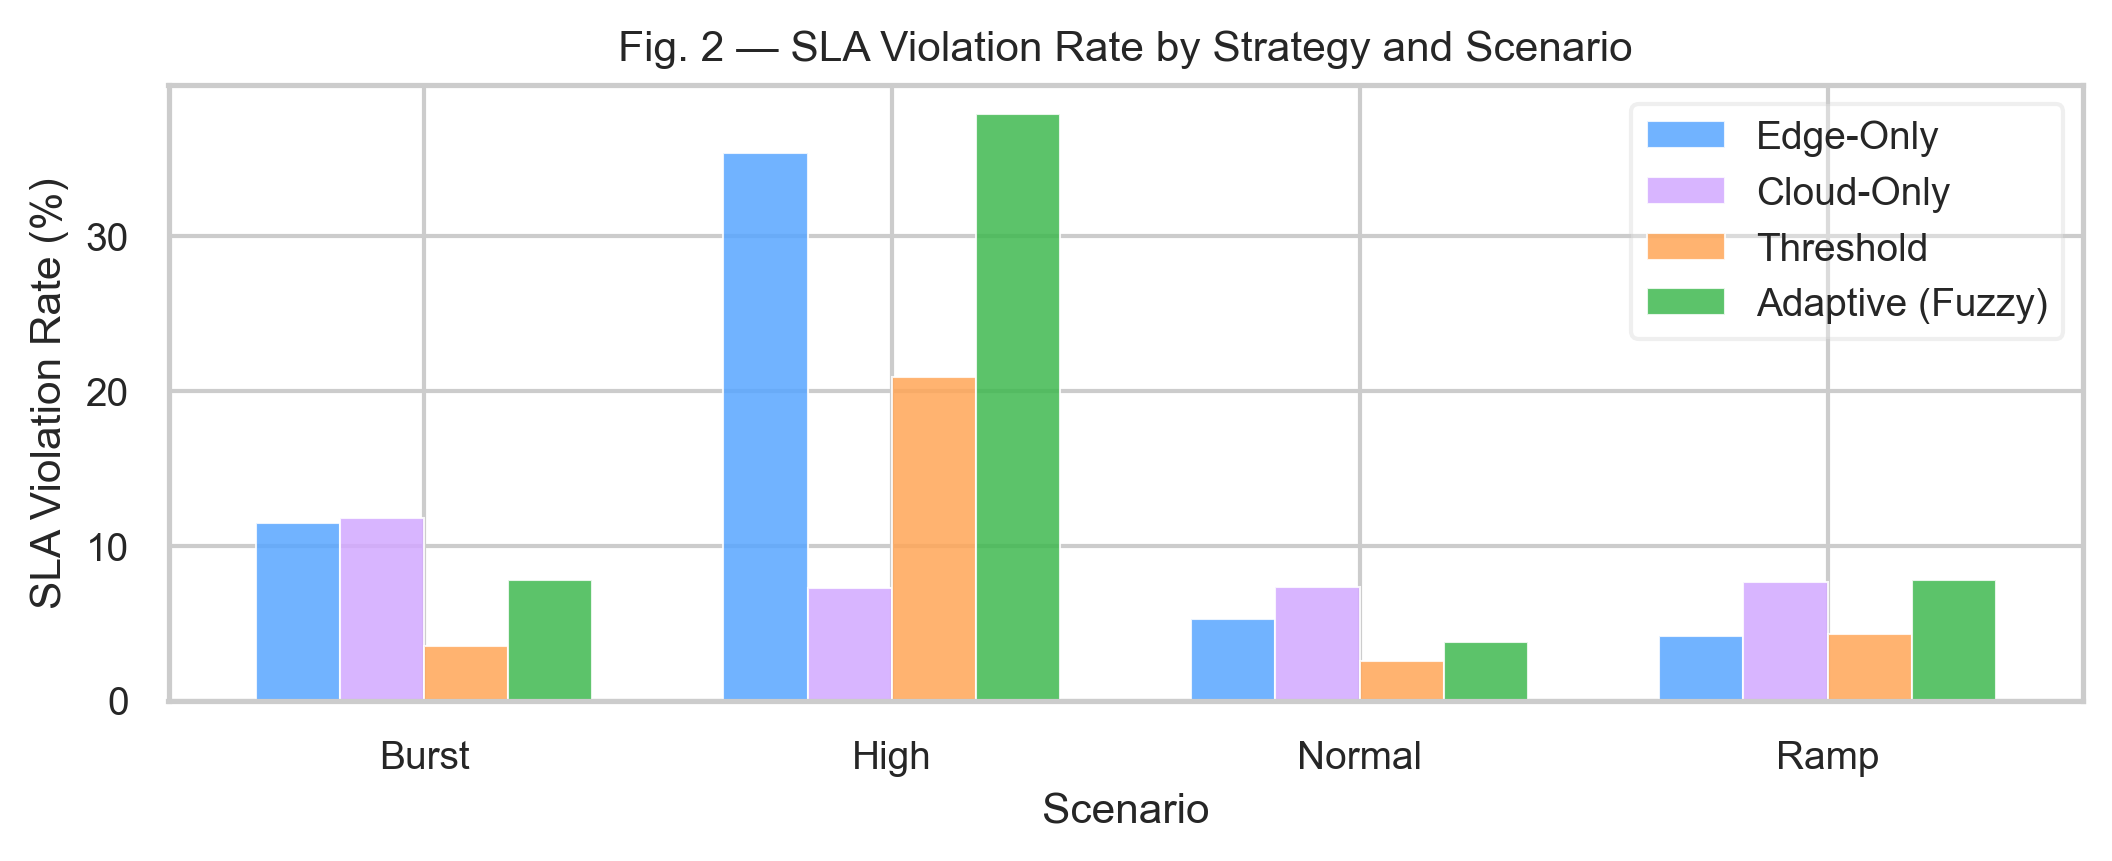
\includegraphics[width=\columnwidth]{fig2_sla_violations.png}
\caption{SLA violation percentages. The Adaptive engine maintains balanced reliability, never suffering the severe violation spikes seen in static baselines.}
\label{fig:sla}
\end{figure}

\subsection{Burst Scenario: Real-Time Load Shedding}
During periodic traffic surges, the Adaptive engine completes 276 tasks compared to 228 for Threshold and 237 for Edge-Only, an improvement of over 16\% to 21\%. It also delivers the lowest mean response time at 188.9~ms. As edge queues build up during a surge, the engine senses the expanding queue backlog and diverts overflow jobs to the cloud until local queues drain. Static baselines lack queue-growth sensitivity and inevitably drop or stall tasks during sudden arrivals.

\begin{figure}[h]
\centering
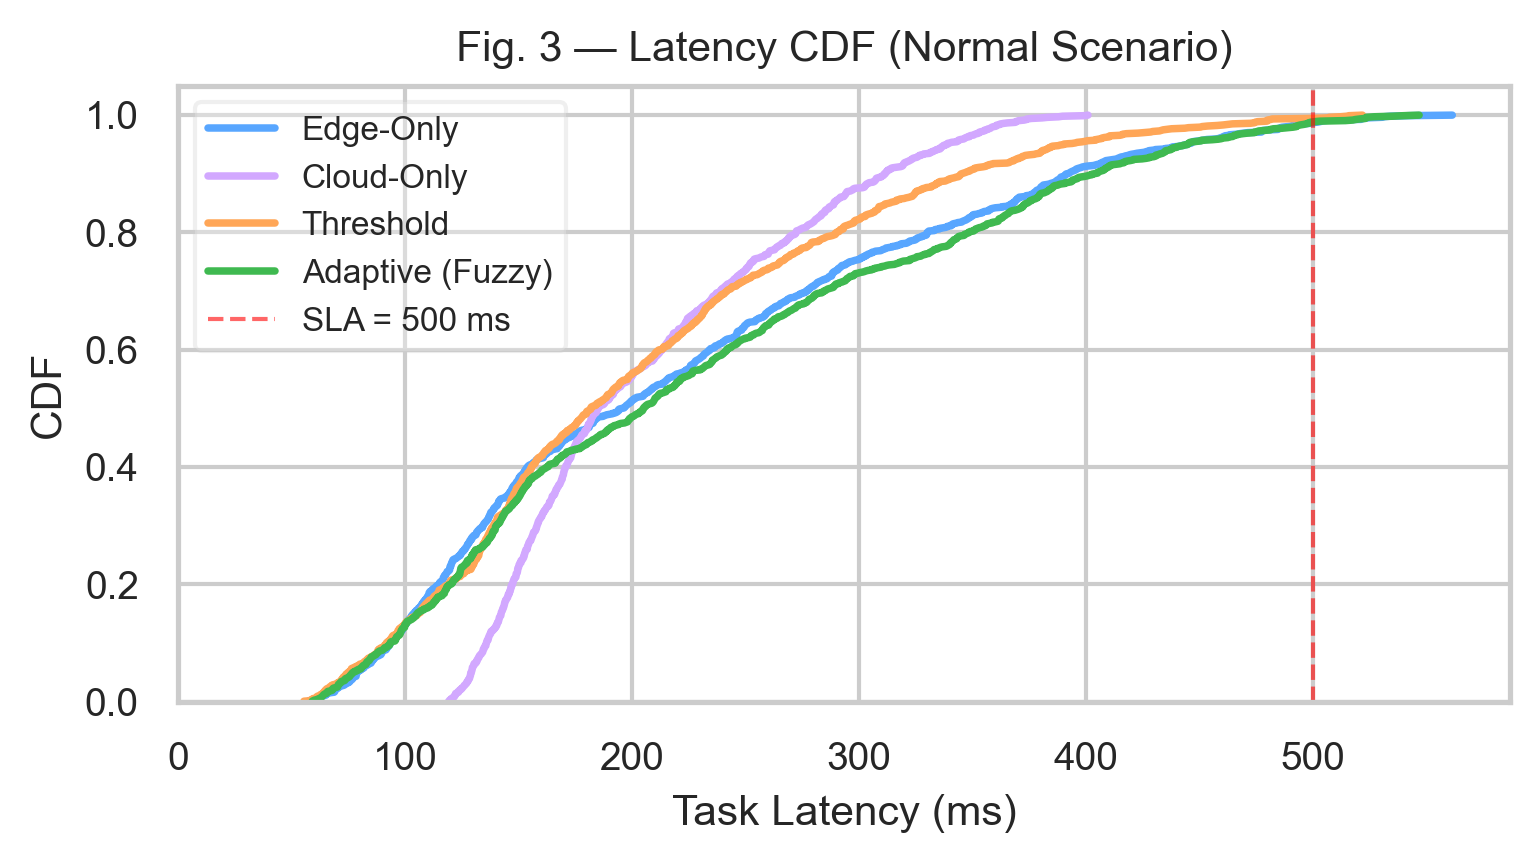
\includegraphics[width=\columnwidth]{fig3_cdf_latency.png}
\caption{Cumulative distribution of response latency under normal traffic. The vertical line at 500~ms indicates the general SLA deadline threshold.}
\label{fig:cdf}
\end{figure}

\subsection{Normal and Ramp Scenarios: Understanding the Trade-off}
In calm, steady-state environments, the Threshold strategy performs best, recording 201.7~ms latency and 3.6\% violations in Normal, and 220.1~ms and 5.1\% violations in Ramp. The Adaptive engine trails by approximately 15\%. This outcome is expected: when traffic is steady and links are healthy, a simple, fixed rule splits tasks by size with zero computational overhead and no boundary misclassifications. The fuzzy model introduces slight evaluation latency and occasionally makes cautious routing choices on borderline inputs.

\begin{figure}[h]
\centering
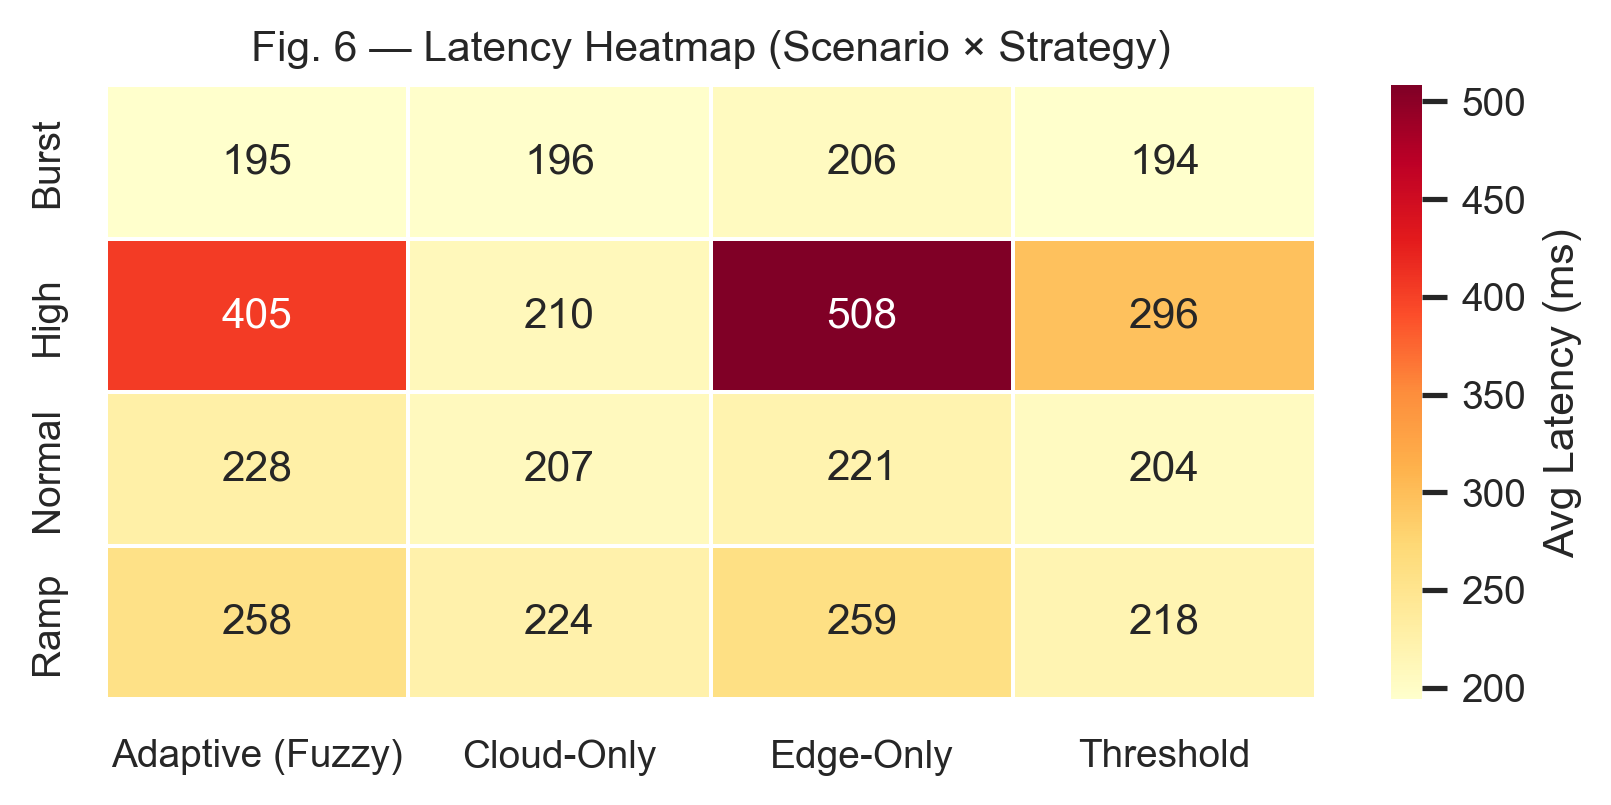
\includegraphics[width=\columnwidth]{fig6_heatmap.png}
\caption{Heatmap of average latency by scenario and strategy. Darker cells highlight severe delays. Edge-Only under High-Latency represents the sharpest bottleneck.}
\label{fig:heatmap}
\end{figure}

\subsection{Cloud Competitiveness Under Moderate Workloads}
Another noteworthy observation is that Cloud-Only execution remains competitive across several tests. A 16-core cloud host running at 3.5~GHz finishes a complexity-5 task in around 28~ms, compared to nearly 57~ms on a 2.0~GHz edge core. That processing speed advantage frequently offsets the 80~ms WAN transit penalty. Edge placement yields a clear advantage only when link latency is genuinely small (under 20~ms) and the local processor has spare capacity.

% ============================================================
\section{Discussion}
\label{sec:discussion}

\subsection{When Adaptive Offloading Delivers Real Value}
Our experimental data highlights two specific regimes where condition-aware offloading is indispensable. First, when network health is variable or degraded, inspecting link quality before every dispatch prevents tasks from being committed to dead-end links. Second, when arrival patterns are bursty, monitoring queue growth allows an orchestrator to offload tasks proactively before servers lock up.

\subsection{A Practical Argument for Hybrid Switching}
Because the Threshold strategy proves slightly more efficient during calm periods, practical production systems should consider a dual-mode hybrid design. A lightweight supervisor can track variance in arrival rates and network latency. When variance is low, the router can execute simple, zero-cost threshold checks. If volatility spikes or links degrade, the supervisor can switch on the full fuzzy inference engine.

\subsection{Lessons from the Physical Override Layer}
In early trials without physical override boundaries, the fuzzy engine produced 495.9~ms average latency under high latency, failing to recognize that local links were degraded because low CPU usage was dominating the score. Introducing deterministic override boundaries immediately corrected this, dropping response times to 202.0~ms. This highlights a valuable engineering takeaway: while fuzzy inference handles ambiguous trade-offs gracefully, deterministic physical rules are essential to enforce hard physical constraints.

\subsection{Energy and Throughput Balance}
Although our engine prioritises latency and deadline satisfaction, energy expenditure remains proportionate. In the Burst scenario, total energy consumed was 964~Ws for Adaptive, compared to 915~Ws for Edge-Only and 782~Ws for Cloud-Only. The modest increase reflects the higher volume of completed tasks (276 versus 228--237) rather than inefficiency on an individual task basis.

\subsection{Limitations and Practical Constraints}
This evaluation uses a discrete-event software simulation with first-order link stochasticity. Real cellular links exhibit multi-path fading, packet loss, and handovers that introduce richer dynamics. Furthermore, our topology models a single cloud cluster and two edge hosts; larger multi-tier environments with heterogeneous accelerators will require broader rule bases. Finally, physical testbed validation on embedded SBC hardware (such as Raspberry Pi clusters) represents an essential next step.

% ============================================================
\section{Conclusion}
\label{sec:conclusion}

This paper presented an adaptive edge-cloud task offloading framework that combines a 12-rule Fuzzy Logic engine with deterministic physical overrides. Evaluated across 22{,}628 simulated task executions across four operational environments, the study yields four clear insights:
\begin{enumerate}
  \item When edge network links suffer severe degradation, adaptive placement reduces average latency by 59.7\% over Edge-Only placement and by 31.0\% over threshold heuristics.
  \item During bursty traffic surges, queue-sensitive dynamic offloading lifts completed throughput by 21\%, preventing local queue overflows.
  \item In steady, predictable environments, well-tuned static rules perform admirably with zero inference overhead, supporting a hybrid two-tier control architecture.
  \item Edge compute nodes are not universally superior to remote clouds; processing speed advantages in large cloud clusters frequently overcome transmission latencies for compute-heavy routines.
\end{enumerate}

Future efforts will focus on replacing manual membership tuning with online Deep Q-Learning, expanding the testbed to larger multi-edge meshes, and deploying the orchestrator on physical edge testbeds.

% ── Acknowledgments ────────────────────────────────────────
\section*{Acknowledgments}
The authors express their gratitude to the faculty and staff of the Department of Information Technology at Kalasalingam Academy of Research and Education for their guidance and institutional support. The simulation platform was constructed using open-source tools including Python, SimPy, scikit-fuzzy, Dash, Plotly, and SQLite.

% ── References ─────────────────────────────────────────────
\bibliographystyle{IEEEtran}
\begin{thebibliography}{10}

\bibitem{mao2017survey}
Y. Mao, C. You, J. Zhang, K. Huang, and K.~B. Letaief,
``A survey on mobile edge computing: The communication perspective,''
\textit{IEEE Commun.\ Surveys Tuts.}, vol.~19, no.~4,
pp.~2322--2358, 2017.

\bibitem{you2016energy}
C. You, K. Huang, H. Chae, and B.-H. Kim,
``Energy-efficient resource allocation for mobile-edge computation offloading,''
\textit{IEEE Trans.\ Wireless Commun.}, vol.~16, no.~3,
pp.~1397--1411, 2016.

\bibitem{chen2016efficient}
X. Chen, L. Jiao, W. Li, and X. Fu,
``Efficient multi-user computation offloading for mobile-edge cloud computing,''
\textit{IEEE/ACM Trans.\ Netw.}, vol.~24, no.~5,
pp.~2795--2808, 2016.

\bibitem{zhang2018joint}
K. Zhang et al.,
``Energy-efficient offloading for mobile edge computing in 5G heterogeneous networks,''
\textit{IEEE Access}, vol.~4, pp.~5896--5907, 2018.

\bibitem{sardellitti2015joint}
S. Sardellitti, G. Scutari, and S. Barbarossa,
``Joint optimization of radio and computational resources for multicell mobile-edge computing,''
\textit{IEEE Trans.\ Signal Inf.\ Process.\ Netw.},
vol.~1, no.~2, pp.~89--103, 2015.

\bibitem{zadeh1965fuzzy}
L.~A. Zadeh,
``Fuzzy sets,''
\textit{Inf.\ Control}, vol.~8, no.~3, pp.~338--353, 1965.

\bibitem{min2019learning}
M. Min, L. Xiao, Y. Chen, P. Cheng, D. Wu, and W. Zhuang,
``Learning-based computation offloading for IoT devices with energy harvesting,''
\textit{IEEE Trans.\ Veh.\ Technol.}, vol.~68, no.~2,
pp.~1930--1941, 2019.

\bibitem{calheiros2011cloudsim}
R.~N. Calheiros, R. Ranjan, A. Beloglazov, C.~A.~F. De Rose, and R. Buyya,
``CloudSim: A toolkit for modeling and simulation of cloud computing environments and evaluation of resource provisioning algorithms,''
\textit{Softw., Pract.\ Exper.}, vol.~41, no.~1,
pp.~23--50, 2011.

\bibitem{gupta2017ifogsim}
H. Gupta, A.~V. Dastjerdi, S.~K. Ghosh, and R. Buyya,
``iFogSim: A toolkit for modeling and simulation of resource management techniques in the Internet of Things, edge and fog computing environments,''
\textit{Softw., Pract.\ Exper.}, vol.~47, no.~9,
pp.~1275--1296, 2017.

\bibitem{matloff2008introduction}
N. Matloff,
``Introduction to discrete-event simulation and the SimPy language,''
Univ.\ California Davis, Dept.\ Comput.\ Sci., 2008.

\end{thebibliography}

\end{document}
